\section{Methods}

\begin{comment}
Here you explain how you’ve solved the problem
in our case

SITUATION: Problem X is very important because . . .
COMPLICATION: In tackling problem X, related work failed in doing Y
PROPOSAL: To partly tackle Y, we make N contributions [list of contributions]

X = organizational moral misalignment
Y = incorporating different perspectives

we solve the problem of incorporating different perspectives
so we explain how we did it
\end{comment}

\subsection{Proposal}
\label{sec:proposal}

To incorporate perspectives of different organizational roles when making company decisions,
we propose a novel software tool.
The tool is intended to be used by company decision makers when taking decisions on internal dilemmas,
with the goal of making more informed decisions.
The user inputs a moral dilemma in the tool, and the tool gives the user a summary as output.
Internally, the tool simulates a deliberation among AI agents representing different organizational roles, on the given dilemma.
A moderator agent poses the dilemma to the other agents, oversees the discussion and finally generates the summary drawing from the deliberation transcript.
The moderator generates the final summary by extracting the key points in which the role-based agents agreed and disagreed during the discussion,
and a list of key points and/or questions that the end user should cover when answering the dilemma.
The summary thus contains three paragraphs: areas of agreement, areas of disagreement and practical points for the user to cover when answering the dilemma.
The purpose of this summary is to make the user think critically about the dilemma
without forcing or inducing a particular point of view,
but rather aiding their thought process and enriching their final response
with aspects they might not consider due to lack of efficient communication with other work figures,
as well as other psychological reasons such as underestimating or misunderstanding the dilemma itself and its implications.
The proposed behavior for this tool is general and can be implemented in various ways: varying the number of agents and their roles, the topology in which they discuss, and the type of moderation they are subjected to.
The following section describes specifically the implementation we developed and tested in the context of this study.

\subsection{Implementation}
\label{sec:implementation}

For this pilot study we decided to implement a simple prototype of the proposed tool for the purpose of testing.
We implemented the AI agents and their deliberation using the Plurals \cite{ashkinaze2025pluralsguidingllmssimulated} framework: a Python library that orchestrates AI agents to allow pluralistic AI deliberations.
Plurals eases the definition of agents, discussion topologies and moderators, and provides an abstraction layer over several LLM API backends.
We used GPT-4.1 as the underlying LLM for each agent and the moderator.
We defined three AI agent personas to represent three specific roles inside a generic technology company: a Chief Executive Officer (CEO), an Ethicist and a generic Engineer.
We used the default moderator persona offered by Plurals: an expert impartial moderator overseeing a given task.
In Plurals, agents can be given a common task which is generally the goal that should be achieved by the simulation.
In our case, the task is to provide and answer to the given dilemma, expressing thoughts and opinions.
The moderator is aware of this task, and generally oversees it according to so-called combination instructions, that are executed when the other agents finished responding.
Agents can deliberate according to several topologies offered by Plurals.
For this prototype we decided to use the Ensemble topology, where each agent speaks independently and without interacting with the others.
We chose this topology to simulate the inclusion of different roles's perspectives with the same priority, as opposed to what happens in top-down ethics reviews or information flow in a company's hierarchical reporting structure.
With the goal of proving the positive effects of exposure to these different perspectives, we refrained from developing complicated deliberations and moderations which, we convened, would be best left to develop in a follow-up co-design study to ours.
As such, we implemented a single round of discussion, that is: agents see the task, they respond, and the moderator executes the combination instructions.
The combinations instructions of the moderator instruct it to generate the final summary to present to the user, as discussed in section \ref{sec:proposal}.
The exact prompts we used are available in the appendix section \ref{sec:prompts}.
Our final implementation is summarized in Figure \ref{fig:impl}.

\begin{figure}[h]
  \centering
  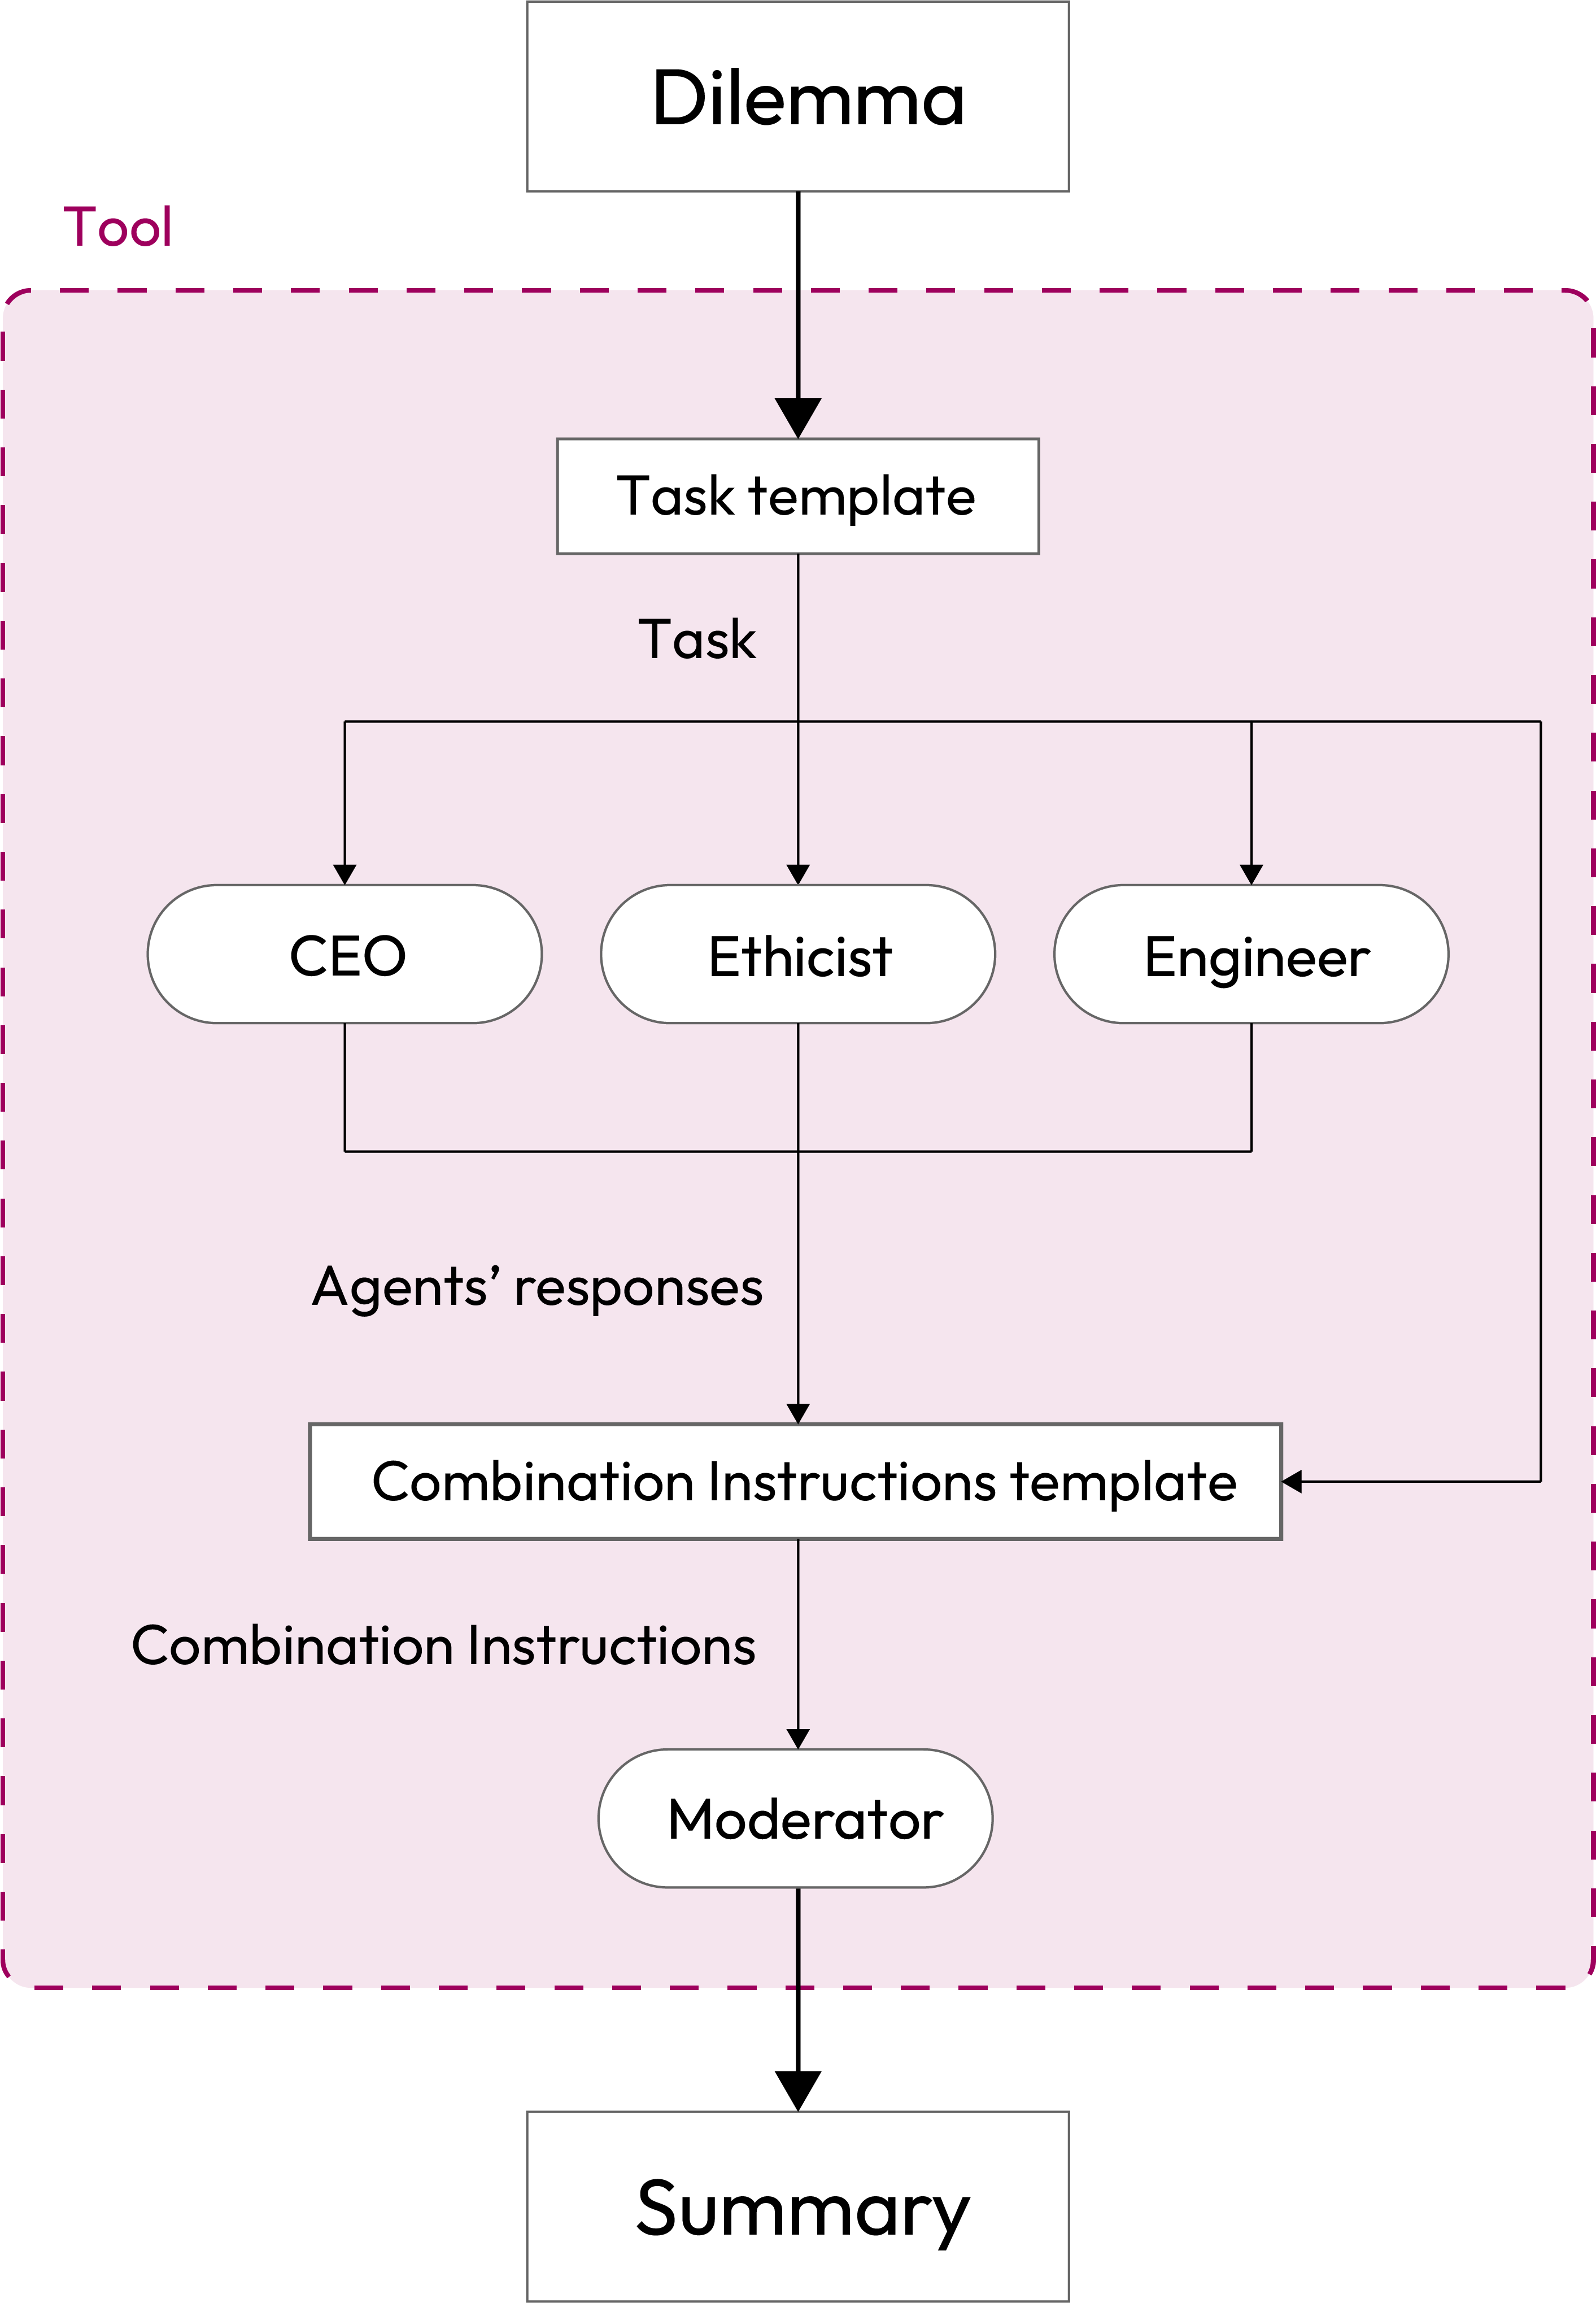
\includegraphics[width=\linewidth]{impl}
  \caption{Implementation of the proposed tool, evaluated in this study. A dilemma is sent as input to the tool. The dilemma is used to build the task for the agents to perform. The three agents give their answer to the task at the same time (Ensemble topology). The agents' responses, together with their task, are used to build the combination instructions for the moderator, which eventually produces the final summary.}
  \Description{Implementation of the proposed tool, evaluated in this study.}
  \label{fig:impl}
\end{figure}
